\documentclass[12pt,a4paper]{report}
\usepackage[utf8]{inputenc}
\usepackage{enumitem}
\usepackage[T1]{fontenc}
\usepackage{ragged2e}
\usepackage{arabtex}
\usepackage{utf8}
\setcode{utf8}
\usepackage{amsmath}
\usepackage{amsfonts}
\usepackage[margin=25mm]{geometry}
\usepackage[compact]{titlesec}
\usepackage{svg}
\usepackage{subcaption}
\usepackage{acronym}
\usepackage{minitoc}
\usepackage{algorithm}
\usepackage{algpseudocode}
\usepackage{footnote}
\usepackage[noadjust]{cite}
\usepackage[section]{placeins}
\usepackage{mathtools}
\usepackage{setspace} 
\usepackage{csquotes}
\newtagform{fn}{(}{)\footnotemark}
\usepackage{multirow}

\usepackage[hyperfootnotes,hidelinks]{hyperref}
\hypersetup{
    linktoc=all
}

\renewcommand{\contentsname}{Table of Contents}

%----------EDIT COVER INFO HERE -----------------%

\def \LOGOPATH {assets/birzeit-logo.png}
\def \UNIVERSITY {Birzeit University}
\def \FACULTY {Faculty of Engineering \& Technology}
\def \DEPARTEMENT {Department of Electrical \& Computer Engineering}
\def \PROJECTTITLE {Accelerated DLRM-based E-commerce Recommendation System}
\def \STUDENTA {Ibraheem Alyan }
\def \STUDENTAID {1201180}
\def \STUDENTB {Mohammad Abu-Shelbaia}
\def \STUDENTBID {1200198}
\def \STUDENTC {Nidal Zabade}
\def \STUDENTCID {1200153}
\def \SUPERVISOR {Dr. Ahmed Shawahna}

%------------------------------------------------%

\begin{document}
\setlength{\parindent}{0em}
\setlength{\parskip}{0.5em}
\setstretch{1.6}
\pagenumbering{Roman}

\begin{titlepage}
    \vfill
    \begin{center}
        \includegraphics[width=0.6\textwidth]{\LOGOPATH} \\
        \fontsize{14pt}{14pt}\selectfont
        \vfill
        % \fontsize{18pt}\textbf{\UNIVERSITY} \\
        \textbf{\FACULTY} \\
        \DEPARTEMENT \\
        \vfill
        \fontsize{17.28pt}{17.28pt}\selectfont
        \textbf{\PROJECTTITLE}
        \fontsize{14pt}{14pt}\selectfont 
        \vfill
        \textbf{Prepared By:} \\
        \STUDENTA \quad \STUDENTAID \\
        \STUDENTB \quad \STUDENTBID \\
        \STUDENTC \quad \STUDENTCID
        \vfill
        \textbf{Supervised By:} \\
        \SUPERVISOR
        \vfill
        A graduation project report submitted to the Electrical and Computer Engineering Department as part of the B.Sc. in Computer Engineering degree requirements fulfillment.
        \vfill
        Birzeit \\
        \today
    \end{center}
\end{titlepage}
\setstretch{1}
\dominitoc

\cleardoublepage \phantomsection \addcontentsline{toc}{chapter}{English Abstract} \mtcaddchapter
\chapter*{Abstract}
The project aims to design and develop a cutting-edge accelerated  e-commerce deep learning recommendation system. The goal is to deliver a production-ready solution, with automated data injestion and training pipelines, and a simple RESTful API as a final interface. The project will have special focus on scalabilty and performance.

This report discusess different types of recommendation systems and compares them to DLRM based systems in terms of different metrics and features. Furthermore, it compares existing solutions and their aspects, and discuesses possible technolgies and architectures to use in the system.
\cleardoublepage \phantomsection \addcontentsline{toc}{chapter}{Arabic Abstract} \mtcaddchapter
\chapter*{\flushright{\RL{المستخلص}}}
\begin{RLtext}
يهدف المشروع إلى تصميم وتطوير نظام توصية لمنصات التجارة الإلكترونية باستعمال التعلم الآلي العميق. الهدف النهائي هو تقديم حلول صالحة لبيئة التشغيل، تتم فيها أتمتة عمليات إدخال البيانات و تدريب نماذج التعلم اللآلي وواجهة برمجة تطبيقات RESTful API كواجهة نهائية. سيركز المشروع بشكل خاص على قابلية التوسع والأداء.

يناقش هذا التقرير أنواعًا مختلفة من أنظمة التوصيات ويقارنها بالأنظمة القائمة على نماذج التوصية بالتعلم اللآلي العميق (DLRM) من حيث المقاييس والميزات المختلفة. علاوة على ذلك، فهو يقارن الحلول المتوفرة حالياً و مزاياها، كما ويناقش التقنيات والبنى الممكن استعمالها في تطوير النظام.
\end{RLtext}

\justifying

\cleardoublepage \phantomsection \addcontentsline{toc}{chapter}{Table of Contents} \mtcaddchapter \tableofcontents

\cleardoublepage \phantomsection \addcontentsline{toc}{chapter}{List of Tables} \mtcaddchapter \listoftables

\cleardoublepage \phantomsection \addcontentsline{toc}{chapter}{List of Figures} \mtcaddchapter \listoffigures

\cleardoublepage

\setlength{\parindent}{0em}
\setlength{\parskip}{0.5em}

\pagenumbering{arabic}

\chapter{Introduction}
\minitoc

\section{Motivation}

The exponential growth of e-commerce has introduced an enormous amount of choice, where consumers face overwhelming product options. To address this challenge, personalized recommendation systems~\cite{raghavendra2018personalized} have become essential for enhancing the shopping experience and increasing the conversion rate for any e-commerce platform.

In contrast to conventional collaborative filtering~\cite{NvidiaRecSys}, content-based~\cite{pazzani2007content}, or popularity-based recommendation systems, our AI-based solution offers distinct advantages. Firstly, AI makes it possible to provide per-user personalized recommendations, which are tailored to their unique preferences and behaviors, enhancing user engagement and satisfaction. AI systems can also intelligently recommend comparable or complementary products or content to increase revenue through cross-selling. Furthermore, AI takes into account the impressions and interactions of users with items, allowing for a more dynamic and accurate understanding of user preferences. Using AI leads to improved recommendation accuracy and relevancy, leading to increased conversion rates and business growth.
    




Statistics from different use cases of recommendation systems:
\begin{itemize}[left=0in]
    \item An intelligent recommender system delivers on average a
    \underline{22.66\% lift in conversions rates}~\cite{salesforce2014predictive} for web products.
    
    \item IKEA experienced a \underline{30\% increase in click-through rate, 2\% surge in average order value}~\cite{IkeaRecAtGoogleCloudSummit} using Google Recommendations AI~\cite{GoogleRecommendationsAI}.
    
    \item Lotte Mart experienced a
    \underline{1.7x increase in new product purchases} ~\cite{LotteMartAwsPersonalize} using Amazon Personalize~\cite{AWSPersonalize}.
\end{itemize}
In summary, the project's motivation is elevating the e-commerce experience, driving business success, and harnessing cutting-edge AI technologies to create a recommendation system that is both high-performing and scalable.

\section{Problem Statement}

The process of building the solution is mainly two parts:

\begin{itemize}
    \item First, designing a personalized recommendation system that covers what traditional collaborative filtering, content-based, or popularity-based systems cannot achieve.
    \item Second, deploying and automating the solution, including, data cleaning, data storage, and model deployment processes, and ensuring a production-ready and scalable system.
\end{itemize}
\section{Report Organization}

The rest of the report is organized as follows. 

Chapter 2 delves into recommendation systems and their components, and reviews related work. 
Chapter 3 outlines functional and system requirements alongside 
a literature review of the existing
recommendation systems and libraries. Chapter 4 unveils the proposed solution, 
its components, and the recommendation pipeline with its stages. 
It also discusses its deployment and infrastructure. 
Chapter 5 presents a Proof-Of-Concept and its results, and analyzes their implications. 
Finally, Chapter 6 
concludes with key findings and outlines promising avenues for 
future exploration.

\chapter{Background}
\minitoc

% \section{Transformer}\label{sec:transformer}

% \subsection{Model Architecture}

% \subsection{Scaled Dot\textendash Product Attention}

% \subsection{Multi\textendash Head Attention}

% \subsection{Self\textendash Attention and Multi\textendash Head Self\textendash Attention}

% \subsection{Feed Forward Network}

% \section{Vision Transformer (ViT)}

% \section{Lightweight ViT}

\section{Recommendation Systems}\label{sec:recommendation-systems}
A recommendation system is an artificial intelligence (AI) technology that provides users with recommendations for items that they may be interested in using Big Data and machine learning techniques. 

Recommender systems undergo training to understand the preferences, earlier decisions, and attributes of the user and products using their past interactions which includes impressions, clicks, purchases, and ratings. Recommender systems are usually used by content and product providers to suggest items to users that they may like based on their profile and preferences. 

\section{Types of Recommendation Systems}\label{sec:types-of-recommendation-systems}
\subsection{Collaborative filtering}\label{subsec:collaborative-filtering}
Collaborative filtering is a technique that can filter out items that a user might like on the basis of reactions by similar users. It works by searching a large group of people and finding a smaller set of users with tastes similar to a particular user. It looks at the items they like and combines them to create a ranked list of suggestions. This technique is based on the idea that people who agreed in the past will agree in the future.
\begin{figure}[H]
    \centering
    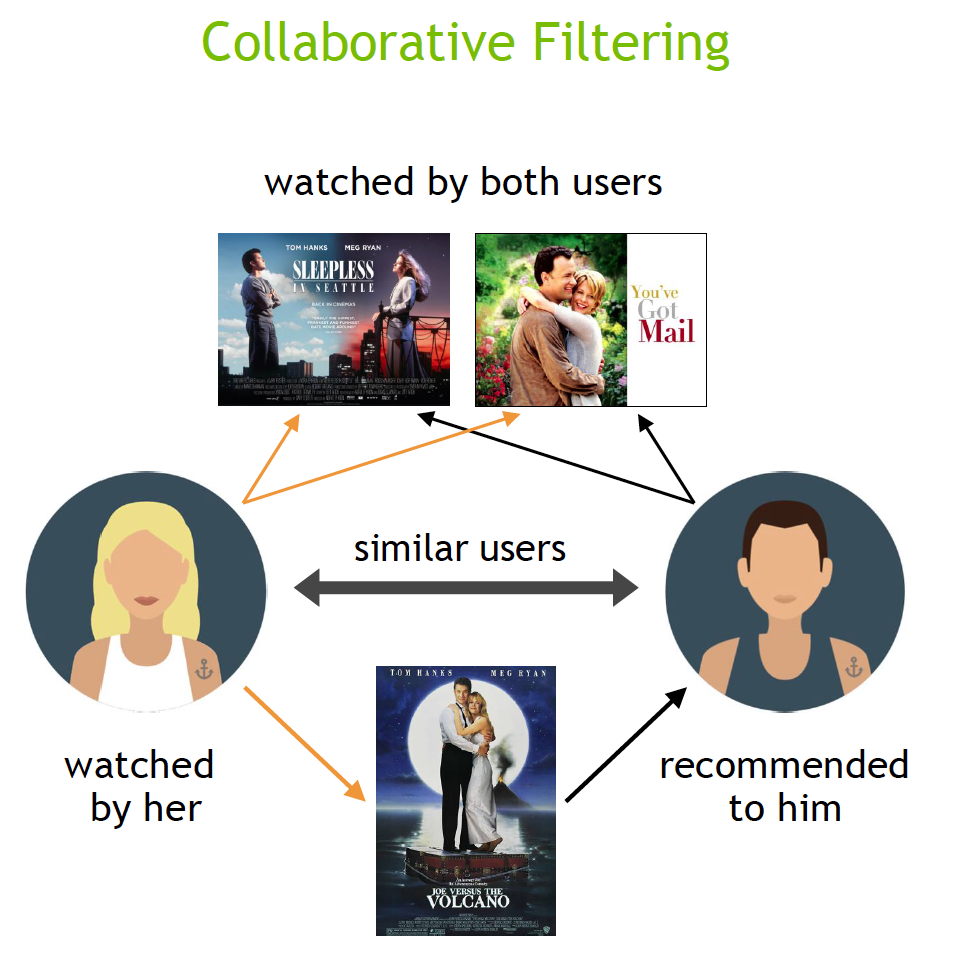
\includegraphics[width=0.4\textwidth]{assets/collaborative_filtering.png}
    \caption{Collaborative Filtering}
    \label{fig:collaborative-filtering}
    \cite{NvidiaRecSys}
\end{figure}

\subsection{Content filtering}\label{subsec:content-filtering}
Content filtering is a technique that uses the features of items a user has interacted with in order to recommend additional items with similar properties. This technique is based on the idea that if a user liked a particular item, he or she will also like an item that is similar to it. 
\begin{figure}[H]
    \centering
    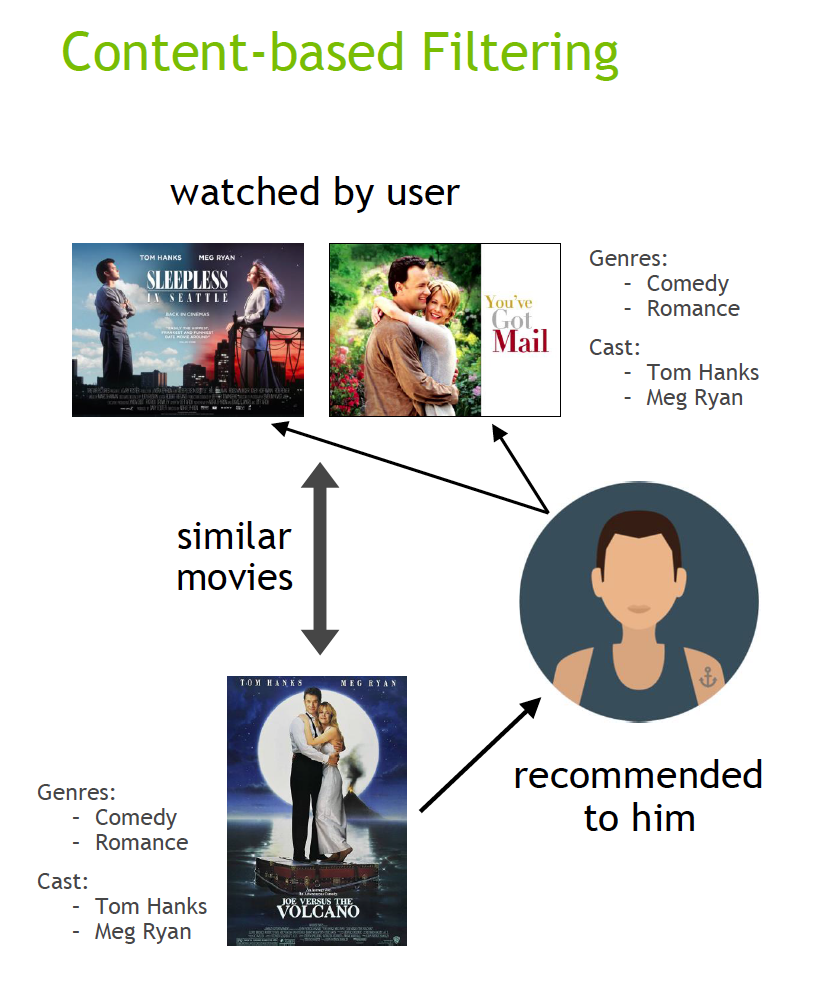
\includegraphics[width=0.4\textwidth]{assets/content_based_filtering.png}
    \caption{Content Filtering}
    \label{fig:content-filtering}
    \cite{NvidiaRecSys}
\end{figure}

\subsection{Hybrid recommendation systems}\label{subsec:hybrid-recommendation-systems}
combine the advantages of the types above to create a more comprehensive recommending system.

\subsection{Context filtering}\label{sec:context-filtering}
Context filtering is a technique that uses the contextual information of the user by framing the recommendation problem as a contextual multi-armed bandit problem and using the contextual information to learn the user's preferences.
\begin{figure}
    \centering
    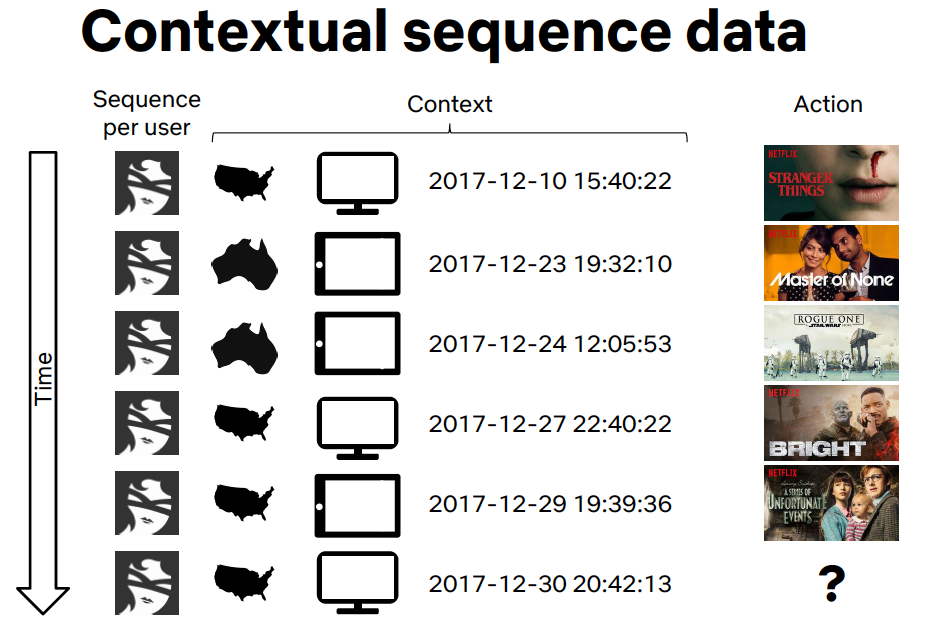
\includegraphics[width=0.5\textwidth]{assets/contextual-sequence-prediction.png}
    \caption{Context Filtering}
    \label{fig:costextual-filtering}
    \cite{NvidiaRecSys}
\end{figure}


\section{DLRM Recommendation System Architecture}

To build a recommendation system based on a deep learning ranking model, there are several stages that the system should go through to provide the final recommendations.

Any system is a group of components that work together to achieve a goal according to a set of rules. The recommendation system is no different, it is a group of components that work together to provide personalized suggestions to users. There are two recommendation system types based on the number of stages they have:
\subsection{Two-stage Recommender Systems}
Two-stage recommender systems are systems that have two main stages: candidate generation and ranking. The candidate generation stage is responsible for generating a set of candidate items for each user, while the ranking stage is responsible for ranking the candidate items and selecting the top items to be recommended to the user. The candidate generation stage is usually based on collaborative filtering or content-based filtering, while the ranking stage is usually based on machine learning models such as matrix factorization or deep learning models.\cite{MultiStageRecSys}
\begin{figure}[H]
    \centering
    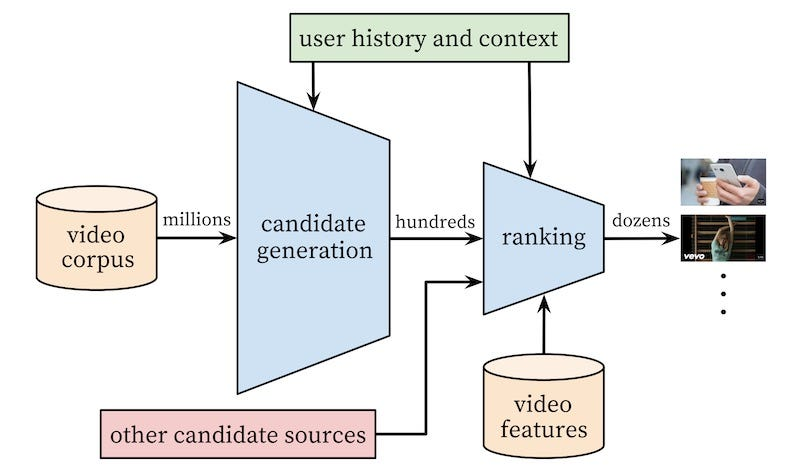
\includegraphics[width=1\textwidth]{assets/Two_stage_rec_sys.jpg}
    \caption[Two-stage Recommender System]{Two-stage Recommender System\cite{MultiStageRecSys}}
\end{figure}
\subsection{Four-stage Recommender Systems}
Four-stage recommender systems are systems that have four main stages: retrieval, filtering, scoring, and ordering. 
The retrieval stage is responsible for retrieving a set of candidate items for each user, 
the filtering stage is responsible for filtering the candidate items according to business rules and constraints,
and the ordering stage is responsible for ordering the scored items and selecting the top items to be recommended to the user. 
The retrieval stage is usually based on collaborative filtering or content-based filtering, while the filtering stage is 
usually based on machine learning models such as matrix factorization or deep learning models, and the scoring and ordering 
stages are usually based on machine learning models such as deep learning models.\cite{NvidiaRecSysBestPractices}
\begin{figure}[H]
    \centering
    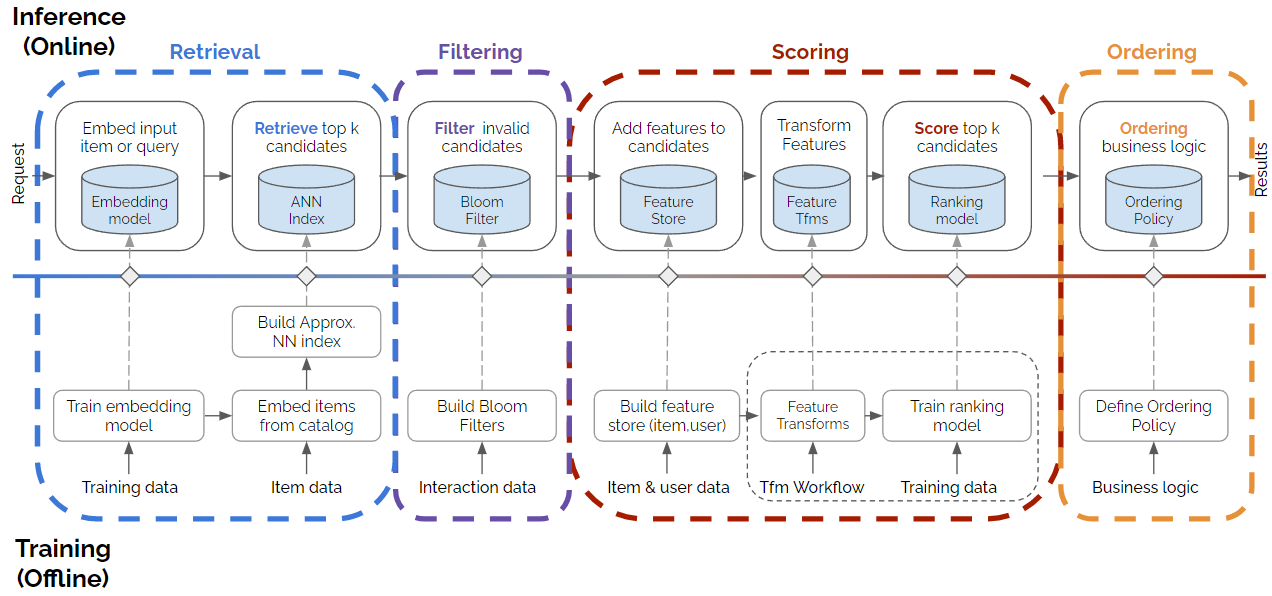
\includegraphics[width=1\textwidth]{assets/Four_stage_rec_sys.png}
    \caption[Four-stage Recommender System]{Four-stage Recommender System\cite{NvidiaRecSysBestPractices}}
\end{figure}
each stage utilizes a set of components and algorithms in training and inference processes to achieve its goal.
\subsection{Trianing (Offline)}
Like any machine learning system, the process of training the models occurs offline,
where the system is trained on a set of historical data, aka batched data, to optimize the model's parameters.
Also in the training phase, the system computes the feature embeddings for all users and items in addition to any other categorical features.


\subsection{Real-Time Inference (Online)}
The inference phase is when the system makes the predictions and suggestions for the application.
To be useful in any website or application, 
the system should be able to provide real-time predictions, 
and suggestions, with a few hundred milliseconds of latency.

In online inference, the system computes the recommendation in Real-time based on the user's interactions and preferences, 
usually with user actions being the trigger for the recommendation generation process.

Figure \ref{fig:TwoStageOnline} shows a pipeline suggested by Nvidia\cite{NvidiaOfflineToOnline} for a two-stage online recommendation system.

\begin{figure}[H]
    \centering
    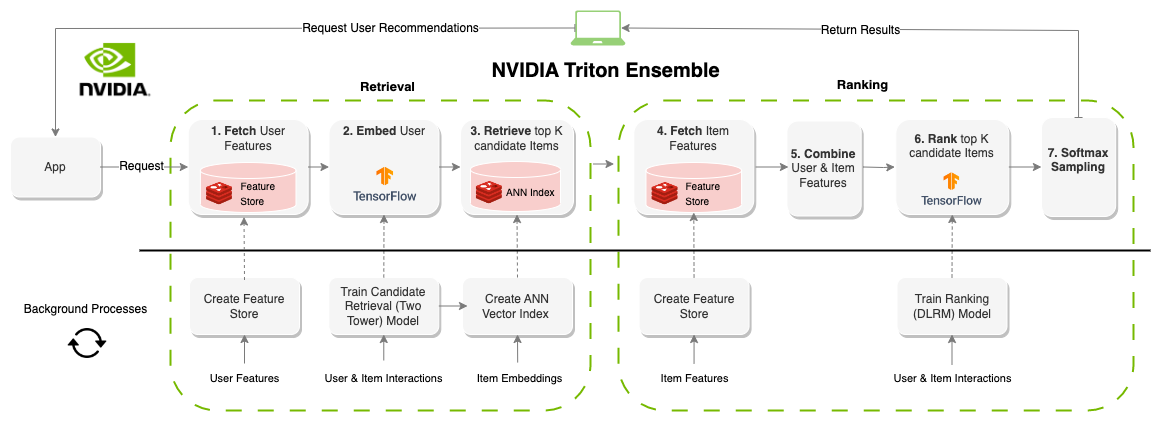
\includegraphics[width=1\textwidth]{assets/online-two-stage-recommender-pipeline.png}
    \caption[Two Stage Online Recommendation System]{Two Stage Online Recommendation System \cite{NvidiaOfflineToOnline}}
    \label{fig:TwoStageOnline}
\end{figure}



\subsection{Batch Inference (Offline)}
Unlike online inference, batch inference is the process of generating recommendations in advance and storing them, 
where the system computes the recommendations for all users and items, 
the process is repeated on a periodical basis.\cite{NvidiaOfflineToOnline} 
Figure \ref{fig:BatchRecSys} illustrates from a high perspective how a completely offline recommendation system operates.

This process allows much shorter response times and is useful for systems with a large number of users and items and a high volume of traffic.

Online and batched inference can be used together to provide real-time recommendations, where the system periodically pre-computes the recommendations for active users, but for new users, the system computes the recommendations in Real-time.



\begin{figure}[H]
    \centering
    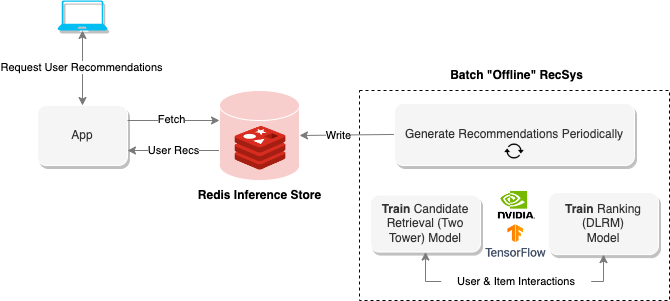
\includegraphics[width=1\textwidth]{assets/batch-recommendation-system.png}
    \caption[Batch Recommendation System]{Batch Recommendation System \cite{NvidiaOfflineToOnline}}
    \label{fig:BatchRecSys}
\end{figure}
\subsection{Retrieval Stage}

To save resources and make a recommendation system effective, the first stage of it is retrieval, 
where the system aims to narrow down the massive 
catalog of items (potentially millions) to a much smaller, 
manageable pool of candidates (around hundreds or thousands).
This initial filtering is crucial because 
directly running the ranking model on every item for every 
user would be computationally expensive and unnecessary.

The recommended approach for retrieval according to Nvidia \cite{NvidiaFeatureStores} is to use a two-tower model in the offline training phase to generate embeddings for users and items.
Then in the online phase ( serving the recommendations ), an ANN search to retrieve the top candidates for each user and use the tower user alone.

\subsubsection{Two-Tower Model}

Another popular approach to retrieval is using a two-tower model, 
The concept for this model design is rather straightforward; as the diagram in Figure \ref{fig: TwoTowerModel} illustrates, it consists of two completely independent towers, 
one for the user and one for the item. 
The model can learn high-level abstract representations for a user and an item 
based on previous user-item interactions thanks to DNN. 

\begin{figure}[H]
    \centering
    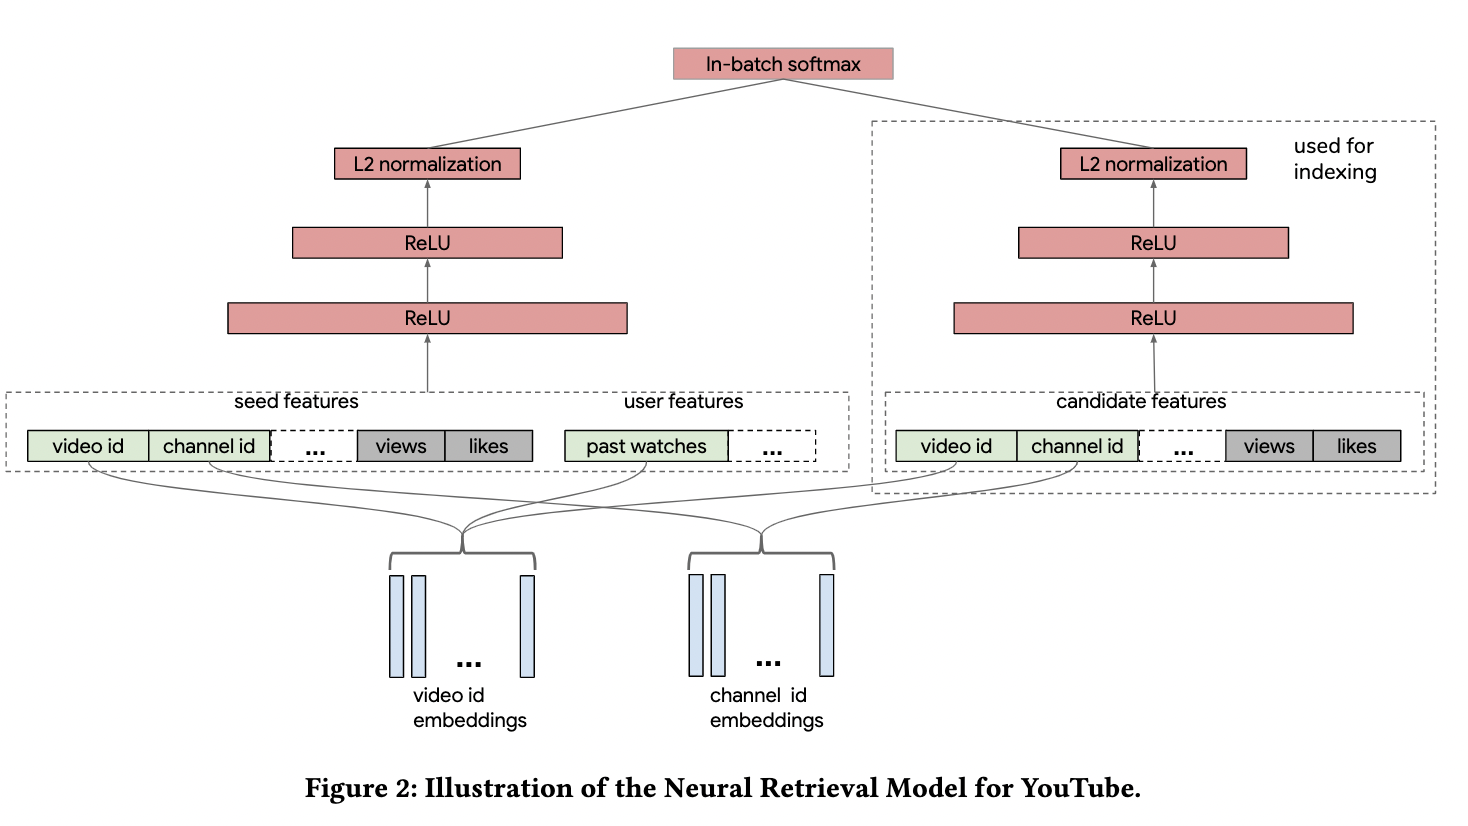
\includegraphics[width=0.9\textwidth]{assets/two_tower.png}
    \caption[Two-Tower Neural Retrieval Model for YouTube]{Two-Tower Neural Retrieval Model for YouTube \cite{YoutubeTwoTower}}
    \label{fig: TwoTowerModel}
\end{figure}

The output of the two-tower model is a vector representing the similarity between item embedding and user embedding, 
it indicates the user's level of interest in the specified item.

Similarity can be either Cosine Similarity, or Euclidean Distance, but cosine is more popular in recommendation systems because it is less sensitive to the magnitude of the vectors, as shown in equation \ref{eq:cosine_similarity}.

\begin{equation}
    \text{Cosine Similarity} = \frac{A \cdot B}{\|A\| \|B\|}
    \label{eq:cosine_similarity}
\end{equation}


\subsubsection{Approximate Nearest Neighbor}

One popular approach to retrieval uses embedding models. 
These models create a dense vector space where users and items are represented as points.
ANN search,
which identifies items closest to the user's representation in the space, 
indicating potential relevance and making them strong candidates for recommendation. figure \ref{fig:AnnVoronoi} illustrates the concept of ANN search. % TODO figure description is wrong FIXME


\begin{figure}[H]
    \centering
    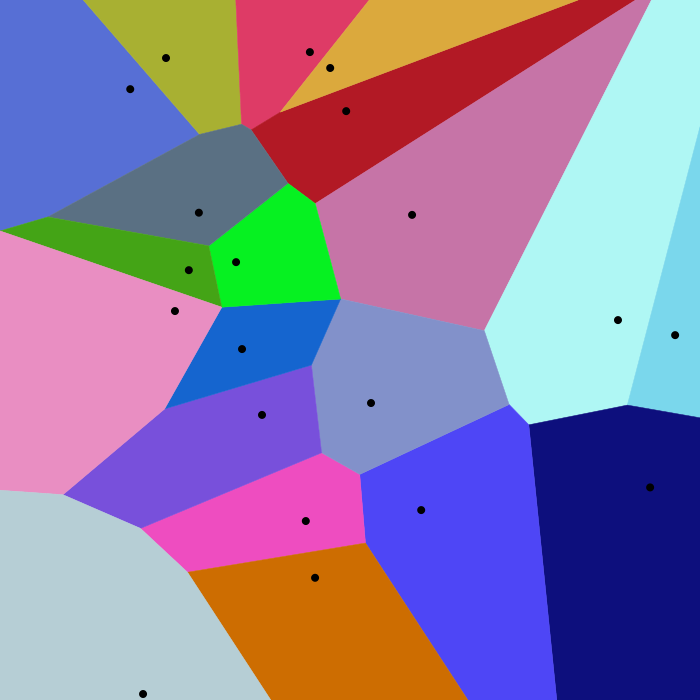
\includegraphics[width=0.35\textwidth]{assets/ann.png}
    \caption[ANN Voronoi Diagram]{ANN Voronoi Diagram \cite{AnnVoronoi}}
    \label{fig:AnnVoronoi}
\end{figure}


\subsection{Filtering Stage}

After retrieving a set of candidate items, the next stage is filtering them according to business rules and constraints.
This stage ensures that only valid candidates are passed to the scoring stage.
For example, products that are out of stock, or products that users already bought.

One possible approach to filtering is using a Bloom filter, which is a space-efficient probabilistic data structure that is used to test whether an element is a member of a set.

Another simpler approach is to use a rule-based system, where the system applies a set of rules to the candidate items to filter out the invalid ones, but it might be less performant than the Bloom filter.


\subsection{Scoring Stage}
% Valid candidates are scored using a richer set of user, item, and session features and a more expressive model such as a deep neural network.

In the scoring stage, valid candidates are scored based on their relevance to the user. Precision in this stage is crucial, more features including user, item, and session features are added that wouldn't have been possibly added in the retrieval stage due to the computational and latency constraints since the retrieval stage processes a large number of items. Moreover, a more expressive model can be used in this stage such as DNN \cite{eugeneyan}. 

Ranking items can be expressed as either a classification problem or a dedicated learning-to-rank problem. In deep learning applications, the final output layer either employs a softmax function to generate preference scores for a set of items or utilizes a sigmoid function to estimate the probability of user interaction (such as clicking or purchasing) for each possible user-item combination \cite{eugeneyan}. 

\subsection{Ordering Stage}
In the ordering stage, We narrow down the choices to the best K options, then adjust their order based on specific business needs. For instance, a product category or manufacturer promotion might influence their ranking \cite{NvidiaRecSysBestPractices}.


\chapter{Requirements And Literature Review}
\minitoc 

\section{Functional Requirements}

The system should provide a RESTful API as the final interface to be used by the front-end application.
The API provides endpoints that allow inserting customers, products, and interactions. In addition to endpoints for retrieving the recommendations for a given customer.

\section{System Requirements}

In order for the system to be useful it has to meet the following specifications:

\subsection{Scalability}
Scalability implies that it has to be cloud-native, the inference system should apply proper load balancing across multi-node, multi-model deployments.

\subsection{Real-time Predictions}
To be usable in any website or application, the system should be able to provide real-time predictions, and suggestions, with a few milliseconds latency. \\

To fulfill this requirement, trained models should run on optimized inference servers or services, the suggested deployment plan is to use
\textbf{Nvidia Triton}
\footnote{Nvidia Triton Inference Server, part of the Nvidia AI platform and available with Nvidia AI Enterprise, is open-source software that standardizes AI model deployment and execution across every workload \cite{Triton}}. 
inference server \cite{Triton}, 
integrated with \textbf{Amazon SageMaker} model deployment \cite{SageMaker} as infrastructure.

\subsection{Near Real-time Training}

This implies continuous training and deployment of the model which requires the automation of training and deployment.

\subsection{Elasticity And Optimization}

Elasticity is vital for keeping up with traffic spikes and declines while optimizing infrastructure costs. To achieve this, the system should be able to scale up and down based on the traffic and load.

\subsection{Security}

Like any other system, the system has to be immune to security threats by implementing best practices at every level in the deployment and design. \\ \\
For example, rate-limiting requests to interaction injection endpoints, using attestation when possible, and limiting access to user and product create, read, update, and delete (CRUD) operations.
 
\section{Related Work}

There are many open-source and paid solutions that provide recommendation systems and libraries, this section discusses some of them.

\subsection{LightFM}
A Python library that enables the classic matrix factorization techniques to include metadata about both items and users, incorporating both content and collaborative information into the recommendation process ( hybrid )\cite{LightFM}.  \\

Its approach is described with more depth in the LightFM paper \cite{kula2015metadata}.

\subsection{Rexy}
Rexy \cite{Rexy} is a Python library that provides a general-purpose recommendation system framework. It is flexible and can be adapted to a variety of data schemas \cite{Rexy}.

\subsection{Gorse}
Gorse \cite{Gorse} is an open-source recommender system engine implemented in Go that provides a scalable and flexible recommendation system framework. It supports a variety of algorithms, including collaborative filtering, content-based filtering, and deep learning \cite{Rexy}.

\subsection{AWS Personalize}
According to Amazon Web Services (AWS), developers can utilize Amazon Personalize \cite{AWSPersonalize} to rapidly create and implement customized recommendations and sophisticated user segmentation on a large scale through machine learning (ML). This service is adaptable to individual requirements, enabling the delivery of personalized customer experiences at the optimal moment and location\footnote{AWS description of the service \cite{AWSPersonalize} }. \\

\subsection{Google Recommendations AI}
As outlined by Google on their cloud marketplace\footnote{Google Cloud Marketplace Recommendations AI Page\cite{GoogleMarketplaceRecAi}}, Recommendations AI \cite{GoogleRecommendationsAI} allows individuals to develop a fully personalized recommendation system utilizing state-of-the-art deep learning ML models, without requiring expertise in ML or recommendation systems. \\

\subsection{Nvidia Merlin}

Nidia defines Merlin \cite{NvidiaMerlin} as "an open source library providing end-to-end GPU-accelerated recommender systems, from feature engineering and preprocessing to training deep learning models and running inference in production." \footnote{Nvidia Merlin Repository \cite{NvidiaMerlinRepo}}. 
\\The frameworks, discussed in more depth later, provide many components including:
\begin{itemize}
    \item Merlin Models \cite{MerlinModels}
    \item Merlin NVTabular \cite{MerlinNVTabular}
    \item Merlin HugeCTR \cite{MerlinHugeCTR}
    \item Merlin Transformers4Rec \cite{MerlinTransformer4Rec}
    \item Merlin SOK (SparseOperationsKit)
    \item Merlin Distributed Embeddings (DE)
    \item Merlin Systems \cite{MerlinSystemsRepo}
\end{itemize}

Making it a very customizable and extensible solution.

\begin{table}[h]
    \centering
    \caption{Comparison of Recommendation Solutions}
    \footnotesize
    \setlength{\tabcolsep}{12pt} % Adjust the spacing between columns
    \renewcommand{\arraystretch}{1.5} % Adjust the spacing between rows
    \begin{tabular}{|l|l|}
        \hline
        \textbf{System} & \textbf{LightFM} \\
        \cline{2-2}
        \textbf{License} & Apache 2.0 \\
        \cline{2-2}
        \textbf{Algorithm Type} & Matrix Factorization \\
        \cline{2-2}
        \textbf{Hardware Utilization} & CPU \\
        \cline{2-2}
        \textbf{Deployment Readiness} & Library (Additional Components Needed) \\
        \cline{2-2}
        \textbf{Notes} & - \\
        \hline
        \hline
        \textbf{System} & \textbf{Rexy} \\
        \cline{2-2}
        \textbf{License} & MIT \\
        \cline{2-2}
        \textbf{Algorithm Type} & Matrix Factorization \\
        \cline{2-2}
        \textbf{Hardware Utilization} & CPU \\
        \cline{2-2}
        \textbf{Deployment Readiness} & Library (Additional Components Needed) \\
        \cline{2-2}
        \textbf{Notes} & - \\
        \hline
        \hline
        \textbf{System} & \textbf{Gorse} \\
        \cline{2-2}
        \textbf{License} & Apache 2.0 \\
        \cline{2-2}
        \textbf{Algorithm Type} & Matrix Factorization \\
        \cline{2-2}
        \textbf{Hardware Utilization} & CPU \\
        \cline{2-2}
        \textbf{Deployment Readiness} & Single-node-learning multi-node-inference cluster \\
        \cline{2-2}
        \textbf{Notes} & Unreliable and has many bugs \\
        \hline
        \hline
        \textbf{System} &\textbf{AWS Personalize} \\
        \cline{2-2}
        \textbf{License} & Proprietary \\
        \cline{2-2}
        \textbf{Algorithm Type} & DLRM \\
        \cline{2-2}
        \textbf{Hardware Utilization} & - \\
        \cline{2-2}
        \textbf{Deployment Readiness} & A lot of customization required  \\
        \cline{2-2}
        \textbf{Notes} & High customization, predictions, and training fees \\
        \hline
        \hline
        \textbf{System} & \textbf{Google Recommendations AI} \\
        \cline{2-2}
        \textbf{License} & Proprietary \\
        \cline{2-2}
        \textbf{Algorithm Type} & DLRM \\
        \cline{2-2}
        \textbf{Hardware Utilization} & - \\
        \cline{2-2}
        \textbf{Deployment Readiness} & End-to-End service \\
        \cline{2-2}
        \textbf{Notes} & High predictions, and training fees \\
        \hline
        \hline
        \textbf{System} & \textbf{Nvidia Merlin} \\
        \cline{2-2}
        \textbf{License} & Apache 2.0 \\
        \cline{2-2}
        \textbf{Algorithm Type} & Multiple Options  \\
        \cline{2-2}
        \textbf{Hardware Utilization} & Optimized for Nvidia GPUs \\
        \cline{2-2}
        \textbf{Deployment Readiness} & Recommendation pipelines components \\
        \cline{2-2}
        \textbf{Notes} & Very customizable \\
        \hline
    \end{tabular}
\end{table}
        
\section{Recommendation System Purpose and Components}
\subsection{Purpose}
The purpose of a recommendation system is to provide personalized suggestions to users based on their preferences and interactions. The system should be able to provide recommendations for new users and items, as well as for existing users and items. The system should also be able to provide real-time recommendations and be able to handle large amounts of data and traffic.
\subsection{Recommendation System Stages}
Any system is a group of components that work together to achieve a goal according to a set of rules. The recommendation system is no different, it is a group of components that work together to provide personalized suggestions to users. There is two recommendation system types based of the number of stages they have:
\subsection*{Two-stage Recommender Systems}
Two-stage recommender systems are systems that have two main stages: candidate generation and ranking. The candidate generation stage is responsible for generating a set of candidate items for each user, while the ranking stage is responsible for ranking the candidate items and selecting the top items to be recommended to the user. The candidate generation stage is usually based on collaborative filtering or content-based filtering, while the ranking stage is usually based on machine learning models such as matrix factorization or deep learning models.\cite{MultiStageRecSys}
\begin{figure}[H]
    \centering
    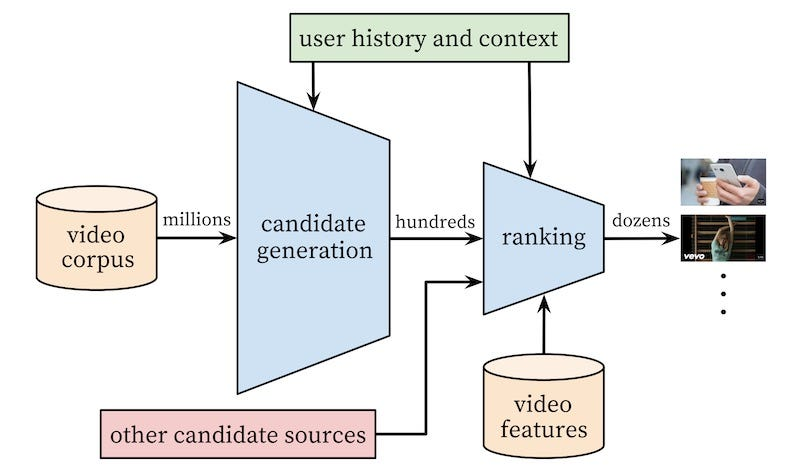
\includegraphics[width=0.7\textwidth]{assets/Two_stage_rec_sys.jpg}
    \caption{Two-stage Recommender System\cite{MultiStageRecSys}}
\end{figure}
\subsection*{Four-stage Recommender Systems}
Four-stage recommender systems are systems that have four main stages: retrieval, filtering, scoring, ordering. The retrieval stage is responsible for retrieving a set of candidate items for each user, the filtering stage is responsible for filtering the candidate items and selecting the top items to be scored, the scoring stage is responsible for scoring the candidate items, and the ordering stage is responsible for ordering the scored items and selecting the top items to be recommended to the user. The retrieval stage is usually based on collaborative filtering or content-based filtering, while the filtering stage is usually based on machine learning models such as matrix factorization or deep learning models, and the scoring and ordering stages are usually based on machine learning models such as deep learning models.\cite{NvidiaRecSysBestPractices}
\begin{figure}[H]
    \centering
    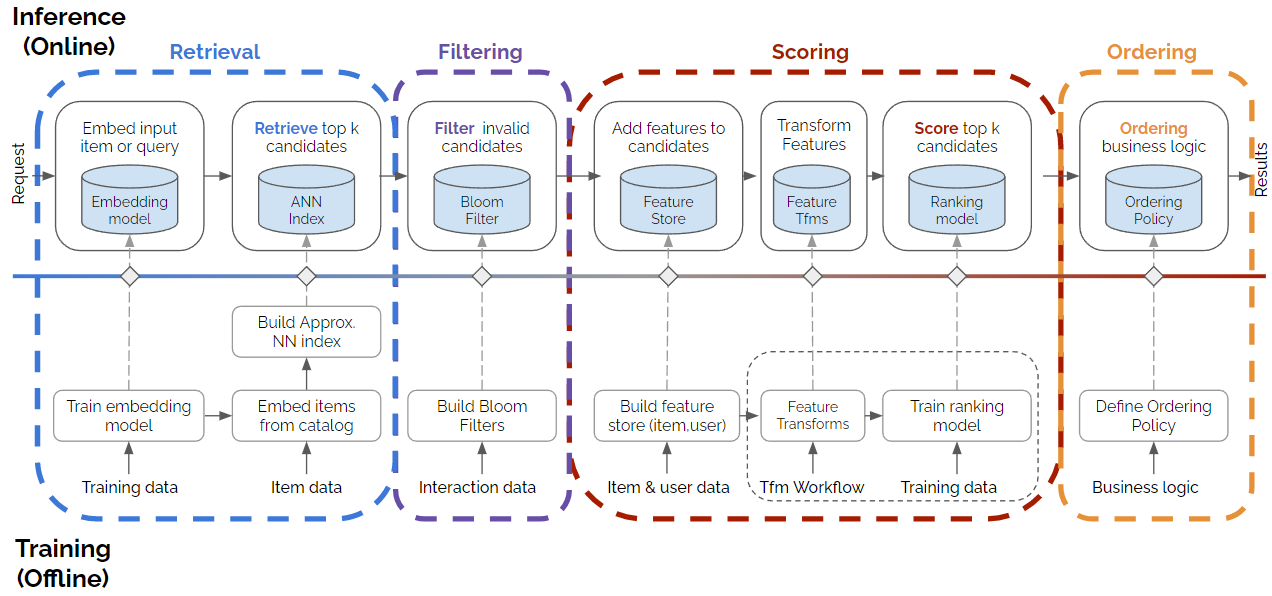
\includegraphics[width=1\textwidth]{assets/Four_stage_rec_sys.png}
    \caption{Four-stage Recommender System\cite{NvidiaRecSysBestPractices}}
\end{figure}
each stage has its own components and algorithms, and divided into two main categories: offline and online components.
\subsection*{Offline Components}
Offline components are components that are responsible for training the machine learning models and generating the recommendation data. The offline components are usually based on batch processing and are responsible for generating the recommendation data in a batch manner.\cite{NvidiaOfflineToOnline}
\subsection*{Online Components}
Online components are components that are responsible for serving the recommendation data to the users. The online components are usually based on real-time processing and are responsible for serving the recommendation data in a real-time manner.\cite{NvidiaOfflineToOnline}
\chapter{Related Work}
\minitoc


\chapter{Solution}
\minitoc

The main goal of this solution is to develop a recommendation system for an e-commerce platform. 
In this context, users are referred to as customers or buyers ( representing individuals interacting with the platform which can be through a website or an app ), 
while products are referred to as items ( representing the goods offered for sale ).

To operate all the stages of the recommendation pipeline and the system components, 
a lot of infrastructure and DevOps work is required, from data ingestion to the deployment of the components, Figure~\ref{fig: SystemComponents} shows a suggested system design by Nvidia.

The following sections will explain the system components and the deployment and technologies used in each stage of the recommendation pipeline.

The system components can be divided into the following categories:
\begin{itemize}
    \item API gateway
    \item Storage Components
    \item Recommendation Pipeline (Offline)
    \item Inference Ensemble (Online)
    \item Caching Layer
    \item Automation and DevOps
\end{itemize}

\begin{figure}[H]
    \centering
    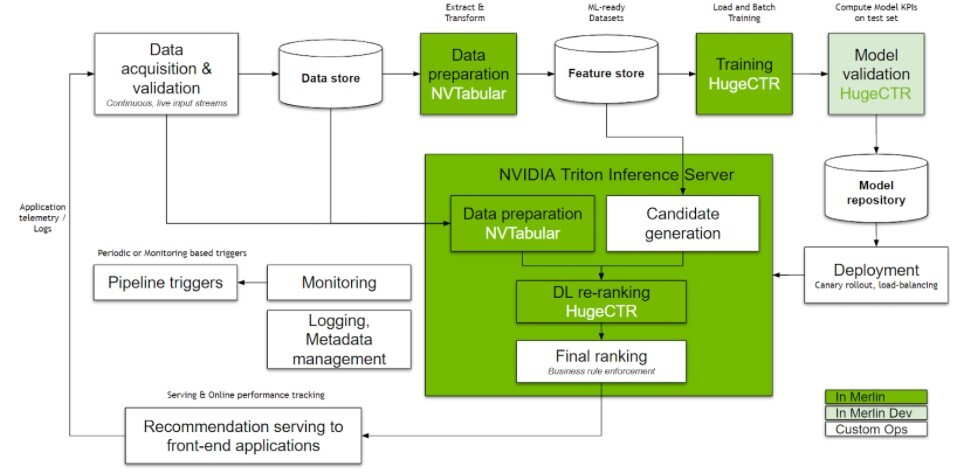
\includegraphics[width=\textwidth]{assets/components.jpeg}
    \caption[System Components]{System Components~\cite{NvidiaRecSysBestPractices}}
    \label{fig: SystemComponents}
\end{figure}

Each component is explained in the following sections.

\section{API Gateway}

The API gateway, a RESTful API, is the entry point for the recommendation system.
It is responsible for handling all the requests and responses from the customers.
The main two functionalities of the API gateway are data ingestion and getting recommendations for a customer.

In addition to these functionalities, the API gateway is also responsible for authenticating and authorizing the requests.

\subsection{Data Ingestion Endpoints}

To handle the data ingestion, the API gateway exposes the following endpoints:
\begin{itemize}
    \item CRUD customers
    \item CRUD products
    \item Adding interactions between customers and products
\end{itemize}

Such endpoints interact mainly with the storage components to store the data.

\subsection{Recommendation Endpoints}

To get recommendations for a customer, the API gateway exposes the following endpoint:
\begin{itemize}
    \item Get recommendations for a customer
    \item Get similar products to a product
\end{itemize}

Those endpoints interact mainly with the recommendation pipeline and the caching layer to get the recommendations.

The first endpoint queries the caching layer to get the recommendations, and if the offline recommendations are not found in the caching layer, 
the API gateway queries the recommendation pipeline to get online recommendations, and then stores the recommendations in the caching layer, 
after getting the recommendations from the recommendation pipeline, 
the API gateway orders the recommendations using the output of the ranking stage and using business rules, then returns the top recommendations to the customer.

In the second endpoint, the API gateway queries a different ensemble that uses the item embedding as a query instead of the user embedding.

\section{Storage Components}

The storage components are responsible for storing the data in different formats and stages, in addition to the models used in the recommendation system.
There are four main storage components in the system:

\begin{itemize}
    \item Main Database
    \begin{displayquote}
        The main database is an SQL database that stores the customers, products, and
         interactions data. In this project, a PostgreSQL~\cite{Postgres} instance 
         deployed using AWS RDS \footnote{AWS Relational Database Service~\cite{AwsRDS}}
         is used as the main database. 
         But in a bigger production environment, a distributed Data Warehouse such as 
         Amazon Redshift~\cite{AwsRedshift} or Google BigQuery~\cite{GoogleBigQuery} can be used.
    \end{displayquote}
    \item Online Feature Store
    \begin{displayquote}
        The feature store is a storage system that stores data in a format optimized for ML models.~\cite{NvidiaFeatureStores}
        It also stores the embedding tables of the customers 
        and products, in addition to any other categorical features.
        This project uses FEAST~\cite{feast} as the feature store, which supports using a Redis~\cite{Redis} 
        cluster as an Online store, the Redis cluster is deployed using AWS ElastiCache~\cite{AwsElastiCache}.
    \end{displayquote}

    \item Item Embedding Store
    \begin{displayquote}
        A vector database that stores the embeddings of the products
        while allowing them to be queried using an ANN search algorithm. 
        In this project, the item embedding store is a Faiss Index\cite{Faiss} that is stored in an S3 bucket and is materialized, loaded in memory, on inference server startup.
    \end{displayquote}

    \item Model Repository
    \begin{displayquote}
        After training the models, their parameters are stored in the model repository. In this project, the model repository is an AWS S3 bucket~\cite{AwsS3}. 
    \end{displayquote}
    \item Results Store
    \begin{displayquote}
       To implement offline batch recommendations, the results of running the recommendation pipeline periodically for all users are stored in the results store. 
       In this project, the results store is a Redis\cite{Redis} cluster deployed using AWS ElastiCache~\cite{AwsElastiCache}.
    \end{displayquote}
\end{itemize}



\chapter{Experiment And Results}
\minitoc

\section{Dataset}

The dataset used in this experiment is called AliCPP and it is a public dataset that contains user-item interactions from an e-commerce platform. The dataset gather traffic logs of recommendation systems in Taobao, a Chinese online shopping website. The dataset is collected from the real-world recommendation system of Taobao.\cite{AliCPP}. The dataset contains of 4 types of features: user features, item features, combination features and context features, each feature is represented by an unique ID, and they described as follows:

\begin{table}[H]
    \centering
    \begin{tabular}{|c|c|c|}
        \hline
        \textbf{Feature Category} & \textbf{Feature ID} & \textbf{Feature Description} \\
        \hline
        \multirow{13}{*}{User Features} & 101 & User ID \\
        \cline{2-3}
        & 109\_14 & User historical behaviors of category ID and count \\
        \cline{2-3}
        & 110\_14 & User historical behaviors of shop ID and count \\
        \cline{2-3}
        & 127\_14 & User historical behaviors of brand ID and count \\
        \cline{2-3}
        & 150\_14 & User historical behaviors of intention node ID and count \\
        \cline{2-3}
        & 121 & Categorical ID of User Profile \\
        \cline{2-3}
        & 122 & Categorical group ID of User Profile \\
        \cline{2-3}
        & 124 & Users Gender ID \\
        \cline{2-3}
        & 125 & Users Age ID \\
        \cline{2-3}
        & 126 & Users Consumption Level Type I \\
        \cline{2-3}
        & 127 & Users Consumption Level Type II \\
        \cline{2-3}
        & 128 & Users Geography Informations \\
        \cline{2-3}
        & 129 & Users Geography Informations \\
        \hline
        \multirow{5}{*}{Item Features} & 205 & Item ID \\
        \cline{2-3}
        & 206 & Category ID to which the item belongs to \\
        \cline{2-3}
        & 207 & Shop ID to which item belongs to \\
        \cline{2-3}
        & 210 & Intention node ID which the item belongs to \\
        \cline{2-3}
        & 216 & Brand ID of the item \\
        \hline
        \multirow{4}{*}{Combination Features} & 508 & The combination of features with 109\_14 and 206 \\
        \cline{2-3}
        & 509 & The combination of features with 110\_14 and 207 \\
        \cline{2-3}
        & 702 & The combination of features with 127\_14 and 216 \\
        \cline{2-3}
        & 853 & The combination of features with 150\_14 and 210 \\
        \hline
        \multirow{1}{*}{Context Features} & 301 & A categorical expression of position \\
        \hline
    \end{tabular}
    \caption{Features Description}
    \label{tab:features}
\end{table}






\section{Experimental Setup}

In order to evaluate the performance of the proposed solution with real-world data, the environment has to be accelerated with a GPU.

\subsection{Hardware Environment}

To achieve this, the experiment is conducted on a cloud-based environment, specifically on an AWS EC2 p3.2xlarge instance \cite{AwsEc2P3}.

The instance is equipped with 8 vCPUs, 61 GiB of memory, and a single NVIDIA Tesla V100 GPU.

The V100 is a high-end GPU that is designed for AI workloads especially deep learning tasks.
It is based on the Volta architecture and is equipped with 5120 CUDA cores, 640 Tensor cores, and 32GB of HBM2 memory with 1.1 TB/s.
It can deliver 7 TFLOPS of double-precision floating-point performance and 116 TFLOPS of deep learning performance.

Figure \ref{fig:V100vsCPU} shows the performance comparison between the Tesla V100 and a CPU.


\begin{figure}[H]
    \centering
    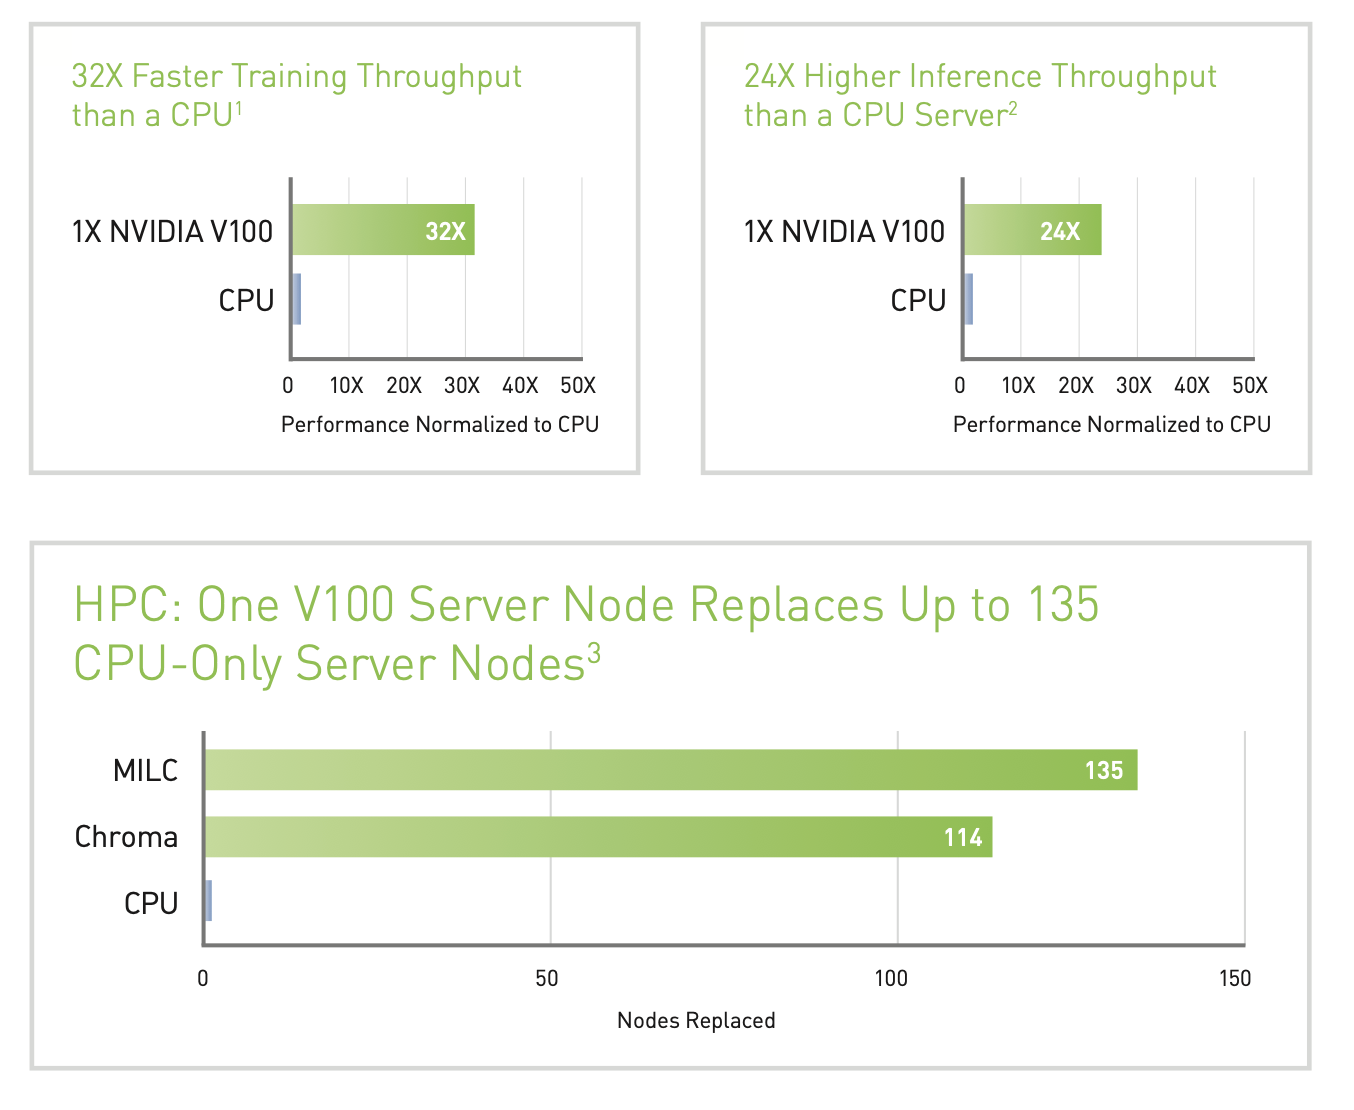
\includegraphics[width=0.8\textwidth]{assets/v100-vs-cpu.png}
    \caption[Tesla V100 vs CPU]{Tesla V100 vs CPU \cite{NvidiaV100DataSheet}}
    \label{fig:V100vsCPU}
\end{figure}

\subsection{Software Environment}

In addition to the hardware environment, the software environment is also important to be considered.
Having access to \textbf{Nvidia Inception Program} \cite{NvidiaStartups}, 
which includes access to NVIDIA AI Enterprise \cite{NvidiaAiEnterprise} with \textbf{Nvidia GPU Cloud (NGC) Catalog}\cite{NvidiaNGC}.

Instead of setting up the drivers, tools, libraries and frameworks manually, 
the Nvidia AI Enterprise provides a pre-configured flavor of Linux Ubuntu that includes all necessities for deep learning tasks.

In addition to that, instead of compiling the Merlin TensorFlow from the source code, 
the Nvidia Merlin TensorFlow Container \cite{NvidiaMerlinTf} was used as a runtime for the experiment Jupyter notebook.


\section{Evaluation Results}
solution is conducted using the AliCPP dataset with various models such as Multi-Layer Perceptron (MLP), Deep Learning Recommendation Model (DLRM), Deep \& Cross Network (DCN), Wide\&Deep, and the Two-Tower model. The evaluation metric used is Area Under the ROC Curve (AUC). Furthermore, we studied the impact of the number of epochs on the training and validation loss and Area Under the ROC Curve (AUC), using Binary Cross-Entropy (BCE) as a loss function.
\subsection{AUC Comparison}

The Area Under the Curve (AUC) metric describes a model's ability to separate positive and negative instances. A higher AUC indicates stronger distinction between the two classes. Where the AUC value ranges from 0 to 1, where 0.5 is the random guess and 1 is the perfect model.

The AUC metric is used to evaluate the performance of the models on the AliCPP dataset. The results are shown in Figure \ref{fig:AUCComparison}.

\begin{figure}[H]
    \centering
    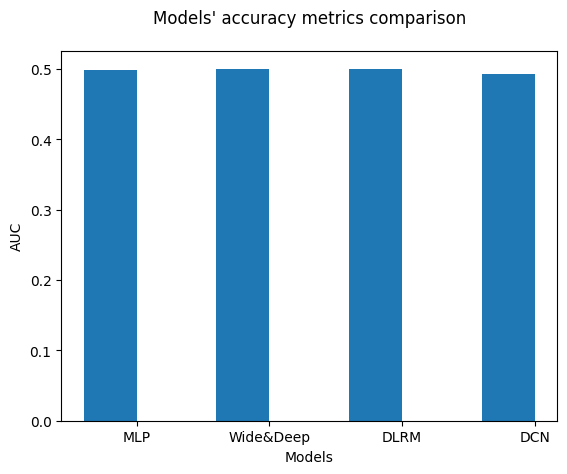
\includegraphics[width=0.6\textwidth]{assets/models_comparasion.png}
    \caption[AUC Comparison]{AUC Comparison}
    \label{fig:AUCComparison}
\end{figure}

The results show that all the models had a similar performance with AUC values around 0.5, which indicates that the models performed similarly.

Recommending relevant items from millions of possibilities is a significant challenge. 
Although an AUC score of 0.5 might seem underwhelming, 
considering it translates to a 50\% chance of the user clicking on a recommended item becomes more impressive. 
Since systems typically show dozens of items, even a single click signifies the success of the system.

\subsection{Training and Validation}

To study the effect of the number of epochs on the training and validation loss and AUC, we trained the models using BCE as a loss function and plotted the AUC, BCE loss for both training and validation datasets over the number of epochs.
The results are shown in Figure \ref{fig:LossComparison} and Figure \ref{fig:AUCOverEpochs}.

The results show that the training loss kept decreasing over the number of epochs, while the validation loss kept increasing, which indicates that the model is overfitting the training data.


\begin{figure}[H]
    \centering
    \begin{subfigure}{.5\textwidth}
        \centering
        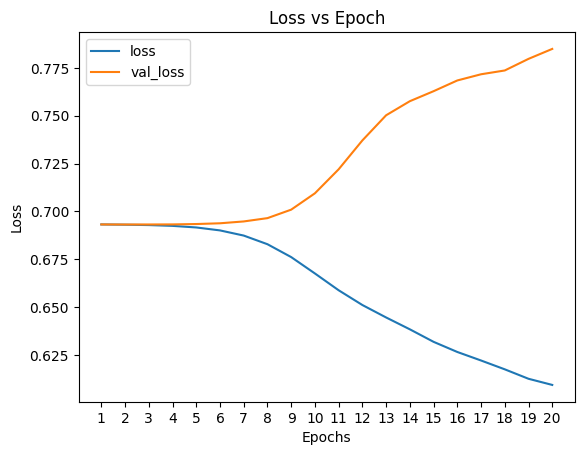
\includegraphics[width=0.95\linewidth]{assets/loss_epochs_20.png}
        \caption[Loss Comparison]{Loss Comparison}
        \label{fig:LossComparison}
    \end{subfigure}%
    \begin{subfigure}{.5\textwidth}
        \centering
        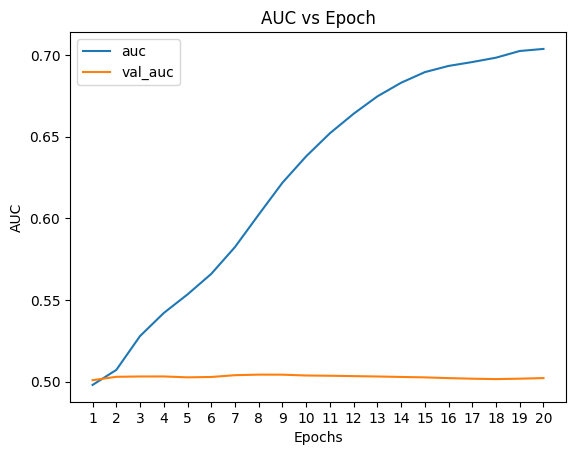
\includegraphics[width=0.95\linewidth]{assets/auc_epochs_20.png}
        \caption[AUC Over Epochs]{AUC Over Epochs}
        \label{fig:AUCOverEpochs}
    \end{subfigure}
    \caption[Measures Over Epoches]{Measures Over Epoches}
\end{figure}


\chapter{Conclusion and Future Work}
\minitoc

\section{Conclusion}

\section{Future Work}

\subsection{Caching Layer}

\cleardoublepage \phantomsection \addcontentsline{toc}{chapter}{Bibliography} \mtcaddchapter
\bibliographystyle{ieeetr.bst}
\bibliography{cites}

\end{document}